\section{Results and Discussion}
\label{sec:Results_and_Discussion}
This section contains lists of all important results and summarizes the most important things.

The following figure \ref{fig:results} shows a graphical comparison between the calculated and the litearture values for the Planck constant $h$.

\begin{figure}[H]
	\centering
	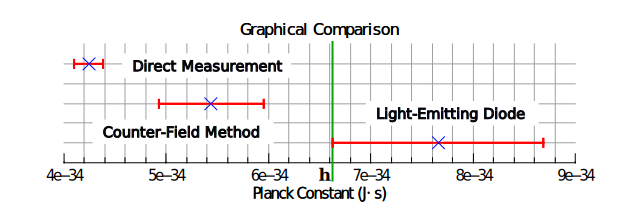
\includegraphics[scale=0.94]{results}
	\caption{Graphcal comparison of the three different methods used to determine the Planck constant $h$. The determined values are shown in blue and the respective uncertainty bars are red. The true value of the Planck constant $h$ is marked in green and annotated with an $h$.}
	\label{fig:results}
\end{figure}

Table \ref{tab:Planck_Constants} shows all calculated Planck constants $h^\prime$ and the literature value of the Planck constant $h$. It is clearly visible that the direct measurement was off the most (>$35\ \%$). The calculated Planck constant $h^{(3)}$ from the threshold voltages of the LEDs was the most precise. The true value of the Planck constant $h$ lies almost inside of the error bar.

\begin{table}[H]
	\centering
	\renewcommand{\arraystretch}{1.2}
	\begin{tabular}{|l|c|}
		\cline{2-2}
		\multicolumn{1}{c|}{} & $\textbf{Planck Constant}\ \boldsymbol{h}$ \\
		\multicolumn{1}{c|}{} & in J$\cdot$s \\
		\hline
		\textbf{Litearture \cite{planck_constant}} & $6.626\cdot10^{-34}$ \\
		\hline\hline
		\textbf{Direct Measurement} & $(4.242\pm 0.140)\cdot10^{-34}$ \\ %424.1812e-036 / 13.9708e-036
		\hline
		\textbf{Counter-Field Method} & $(5.437\pm 0.512)\cdot10^{-34}$ \\ %543.7227e-036 / 51.2277e-036
		\hline
		\textbf{Light-Emitting Diode} & $(7.659\pm 1.032)\cdot10^{-34}$ \\ %765.9386e-036 / 103.1796e-036
		\hline
	\end{tabular}
	\caption{List of all calculated Planck constants $h^\prime$ and the literature value of the Planck constant $h$. The measurement with the LEDs resulted in the most precise value for the Planck constant.}
	\label{tab:Planck_Constants}
\end{table}

It is only possible to determine the Planck constant $h$ through experiments. This not so trivial task had to be fulfilled to successfully redefine the kilogram in the last couple of years.
